\section{Numerical Tests}\label{se:NumericalTests}

In this section we present the numerical results obtained with the PD-ARS schemes given in Section~\ref{se:TimeIntegration}.
The tests in Section \ref{se: Accuracy Tests} are designed to compare the accuracy of the schemes in streaming, absorption, and scattering-dominated regimes in one spatial dimension.
The test in Section \ref{se: Neutrino Stationary State Test} demonstrates the convex-invariance of PD-ARS schemes schemes.
All the tests in this subsection were constructed with third-order accurate spatial discretization (polynomials of degree $k=2$) and time step $\dt = 0.1 \times \dx $.

\subsection{Accuracy Tests}
\label{se: Accuracy Tests}
To compare the accuracy of the IMEX schemes, we applied our PD-ARS schemes and Pareschi \& Russo \cite{pareschiRusso_2005} (SSP2332) scheme to some problems with known smooth solutions in streaming, absorption, ans scattering-dominated regimes in one spatial dimension.
All the tests in this subsection were constructed with the maximum entropy closure in the low-occupancy limit(i.e., the Minerbo closure).
In the streaming test, the second- and third-order accurate explicit strong-stability-preserving Runge-Kutta methods\cite{gottlieb_etal_2001} (SSPRK2 and SSPRK3, respectively) are plotted as references.
To compare the numerical results to analytic solutions, the cell-averaged absolute error or the cell averaged relative error are computed.
For our convergence test, the number of elements ($N$) vary from 8 to 128.

\subsubsection{Sine Wave Streaming}
The sine wave streaming test is designed for the steaming dominated regime, with $\sigma_{\Ab} = \sigma_{\Scatt} = 0$.
A periodic domain with length=1 is used and the initial condition is $\cJ = \bcH =$ a spatial sine wave function.
We evolve the test until the sine wave has completed 10 crossings of the domain.
Figure~\ref{fig: SineWaveStreaming} plots the absolute error for the number density versus the number of elements $N$.
We see the errors obtained with SSPRK3 and PD-ARS with SSPRK3 as the explicit part decrease as $N^{-3}$, as expected.
All the other schemes have errors decreasing as $N^{-2}$.
Among the second-order schemes, SSP2332 has the smallest error.

In the streaming limit, PD-ARS scheme limit to its explicit part, SSPRK2 and SSPRK3, respectively.
That's why the absolute errors of PD-ARS and SSPRK are indistinguishable on the plot.

\begin{figure}[h]
  \centering
    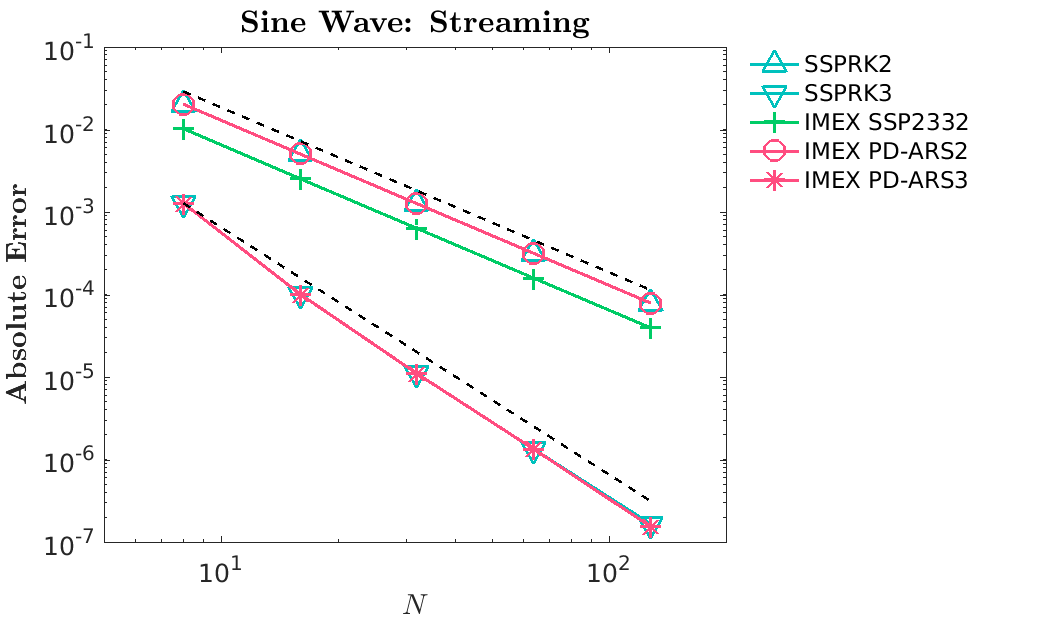
\includegraphics[width=0.8\textwidth]{figures/SineWaveStreaming}
   \caption{Absolute error versus number of elements $N$ for the streaming sine wave test.  Results employing various time stepping schemes are compared: SSPRK2 (cyan triangles pointing up), SSPRK3 (cyan triangles pointing down), SSP2332 (green crosses), PD-ARS with SSPRK2 (light red circles) and PD-ARS with SSPRK2 (light red hexagrams). Black dashed reference lines are proportional to $N^{-2}$ (top), and $N^{-3}$ (bottom), respectively.}
   \label{fig: SineWaveStreaming}
\end{figure}

\subsubsection{Sine Wave Damping}
This test, adapted from \cite{skinnerOstriker_2013}, is designed for absorption-dominated regimes, with $\sigma_{\Scatt} = 0$ and $f_0 = 0$, which results in exponential damping of the wave amplitude.
A periodic domain with length=1 and an initial condition with $\cJ = \bcH =$ a spacial sine wave function is used.
The amplitude of the analytical solution decreases as $e^{-\sigma_{\Ab} t}$.
For $\sigma_{\Ab}$ = 0.1, 1 and 10 we evolve the test until the initial condition has been damped by a factor $e^{-10}$. 
Figure~\ref{fig:SineWaveDamping} shows convergence results of the sine wave damping test in the relative error.
SSP2332, a second-order scheme, displays second-order convergence.
PD-ARS schemes converge with a first-order convergence rate given the price paid for convex-invariance.
\begin{figure}[h]
  \centering
    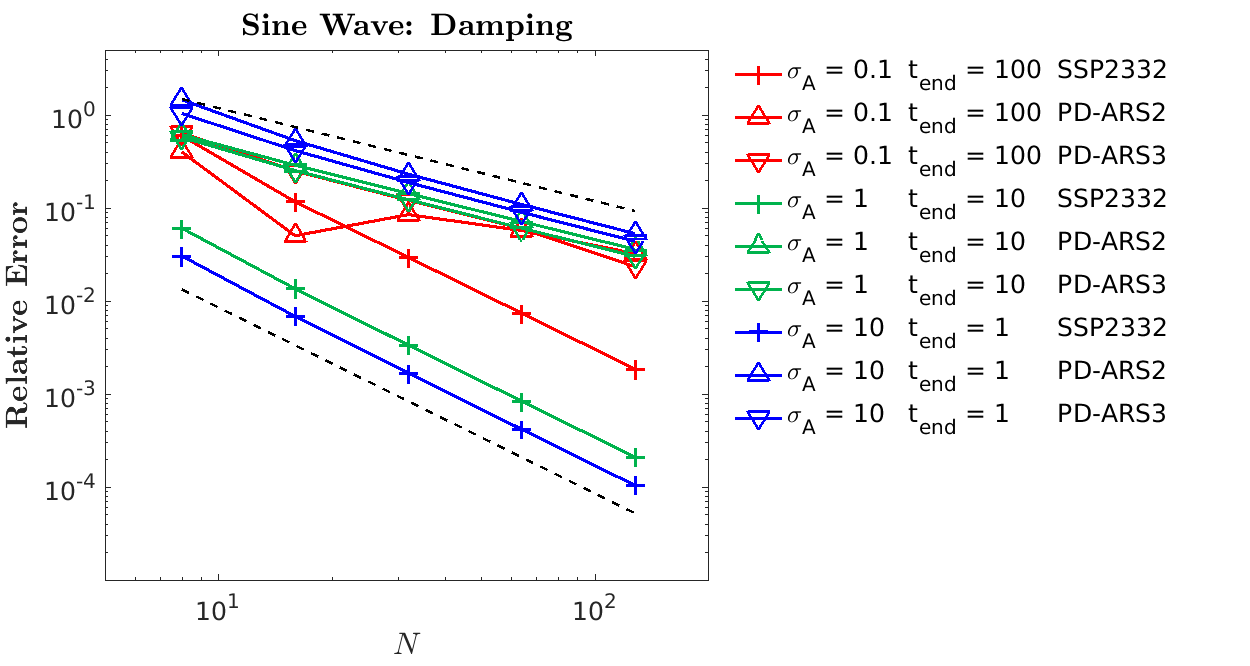
\includegraphics[width=0.9\textwidth]{figures/SineWaveDamping}
   \caption{Relative error versus number of elements, $N$, for the damping sine wave test. Results for different values of the absorption opacity $\sigma_{\Ab}$, employing various IMEX time stepping schemes, are compared.  Errors for $\sigma_{\Ab}=0.1$, $1$, and $10$ are plotted with red, green, and blue lines, respectively.  The IMEX schemes employed are SSP2332 ($+$), PD-ARS with SSPRK2 (circles) and PD-ARS with SSPRK3 (hexagram).  Black dashed reference lines are proportional to $N^{-1}$ (top) and $N^{-2}$ (bottom), respectively.}
  \label{fig:SineWaveDamping}
\end{figure}

\subsubsection{Sine Wave Diffusion}
The last test with known smooth solution,adopted from \cite{radice_etal_2013}, is the sine wave diffusion test with $\sigma_{\Ab} = 0, f_0 = 0$.
A periodic domain with $D=\{x:x\in[-3,3]\}$ and an initial condition with $\cJ_{0}$ = a spatial sine wave function and $\cH =-\f{1}{3\sigma_{\Scatt}}\pderiv{\cJ}{x}$ is used.
The analytic solution is given by $\cJ = \cJ_{0} \times e^{-\f{\pi^2 t}{27\sigma_{\Scatt}}}$ and $\cH = (3\,\sigma_{\Scatt})^{-1}\pd{\cJ}{x}$.
We evolve with $\sigma_{\Scatt}=10^{2}$, $10^{3}$, and $10^{4}$, and adjust the end time so that $t_{\mbox{\tiny end}}/\sigma_{\Scatt}=1$. 
Then the amplitude of the sine wave has been reduced by a factor $e^{-\pi^{2}/27}\approx0.694$ for all values of $\sigma_{\Scatt}$. 
Figure~\ref{fig:SineWaveDiffusionJ} shows the convergence.
SSP2332 and PD-ARS schemes display third-order accuracy for the number density, $\cJ$, and second-order accuracy for $\cH_{x}$, and their errors are difficult to distinguish.
PD-ARS with SSP2332 behaves as good as SSP2332 in the diffusion region but requires 1/3 less implicit solvers.
\begin{figure}[h]
  \centering
  \centerline{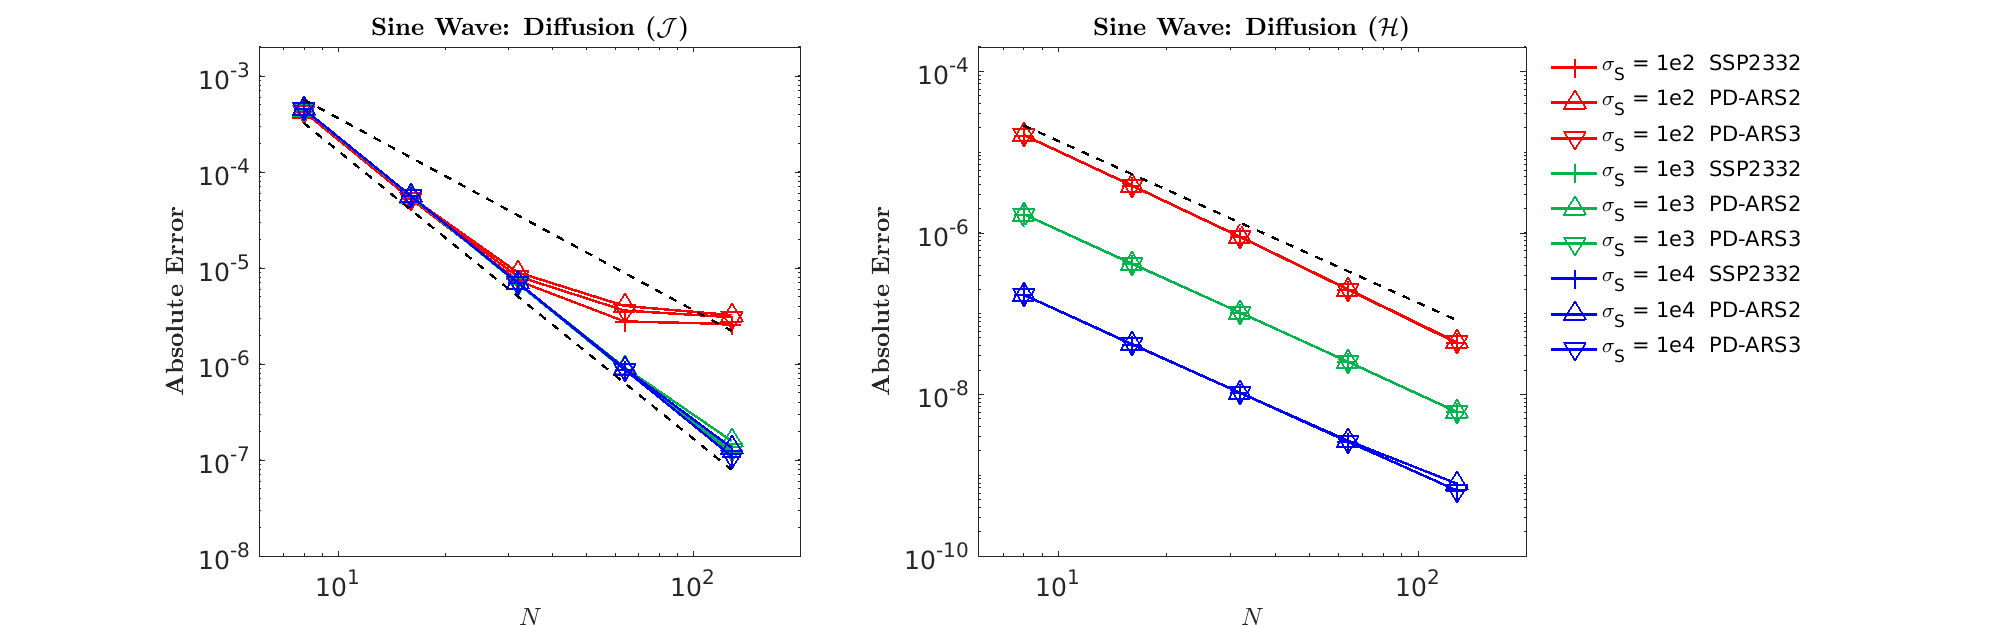
\includegraphics[width=1.2\textwidth]{figures/SineWaveDiffusion}}
%  \begin{tabular}{cc}
%    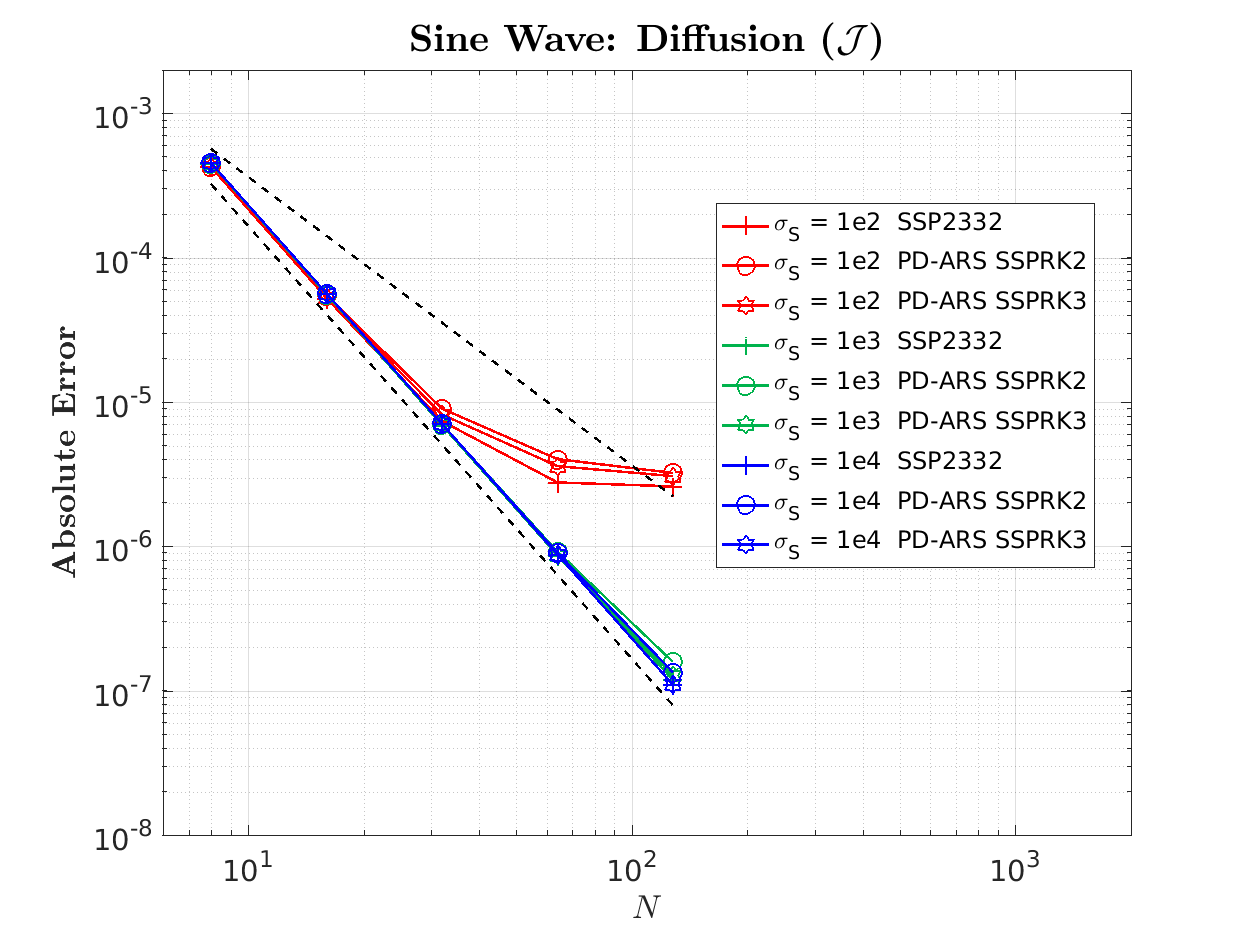
\includegraphics[width=0.5\textwidth]{figures/SineWaveDiffusionJ}
%    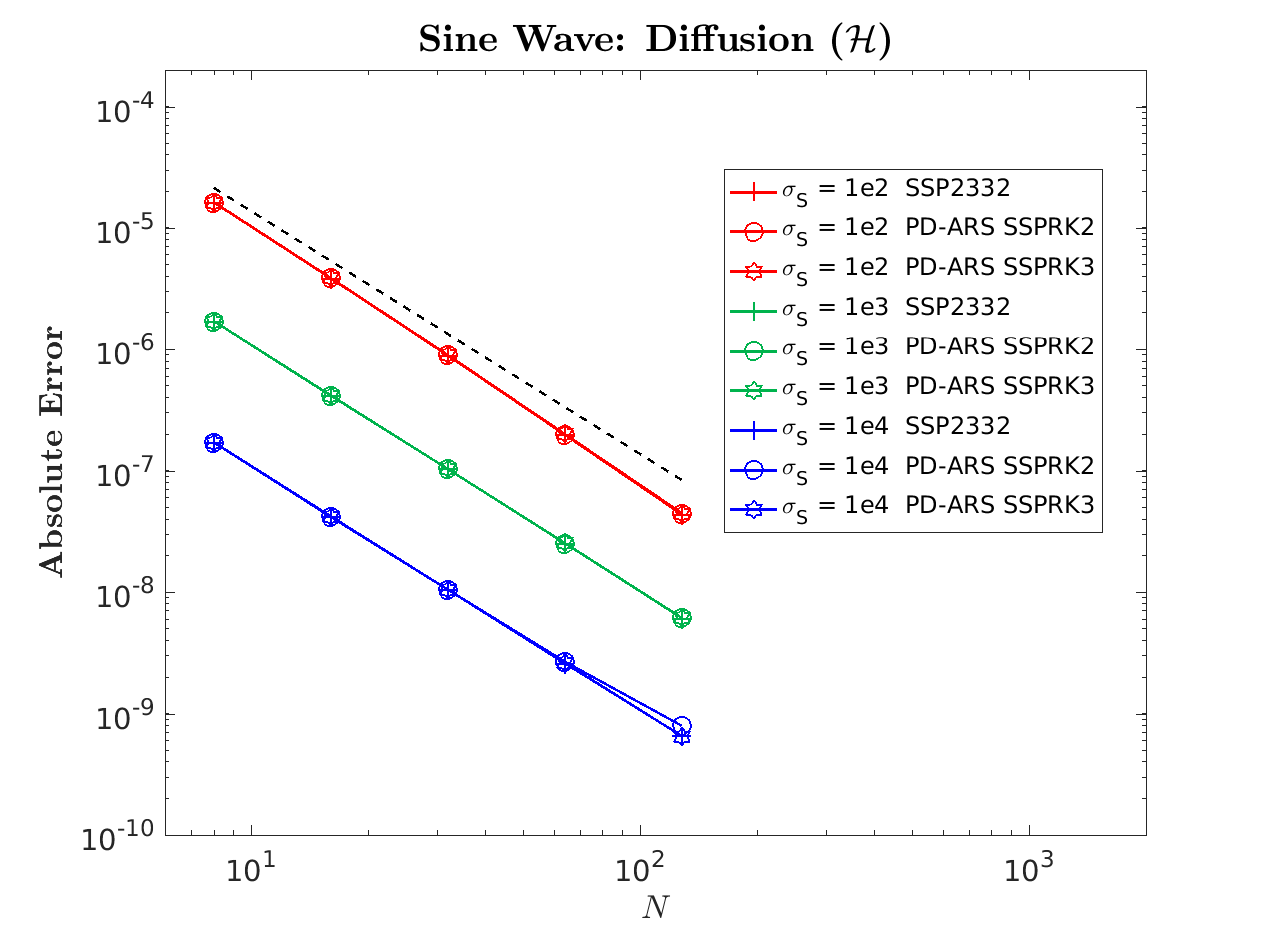
\includegraphics[width=0.5\textwidth]{figures/SineWaveDiffusionH}
%  \end{tabular}
   \caption{Absolute error for the number density $\cJ$ (left) and the number flux $\cH_{x}$ (right) versus number of elements for the sine wave diffusion test.  Results with different values of the scattering opacity $\sigma_{\Scatt}$, employing different IMEX schemes, are compared.  Errors with $\sigma_{\Scatt}=10^{2}$, $10^{3}$, and $10^{4}$ are plotted with red, green, and blue lines, respectively.  The IMEX schemes employed are:  SSP2332 ($+$), PD-ARS with SSPRK2 (circles), and PD-ARS with SSPRK3 (hexagram). Black dashed lines on the left plot reference lines proportional to $N^{-2}$ (top) and $N^{-3}$ (bottom), respectively. Black dashed line on the right plot reference lines proportional to $N^{-2}$ .}
   \label{fig:SineWaveDiffusionJ}
\end{figure}

\subsection{Neutrino Stationary State Test} \label{se: Neutrino Stationary State Test}
Next we consider a more ``realistic'' test: two-dimensional neutrino transport with emission, absorption, and elastic scattering in a stationary ``realistic'' background.
This is designed to test the realizability-preserving properties of the PD-ARS schemes.
Figure~\ref{fig:NeutrinoStationaryTestEOS} plots the thermal state and the opacities we used.
This test is constructed on a two-dimensional domain $D=\{\vect{x}\in\bbR^{2}:x^{1}\in[0,200], x^{2}\in[0,200]\}$ with a grid of 128 elements in each direction.
We take 10 energy groups from 0~MeV to 300~MeV and initialize the neutrino number density $\cJ$ and flux density $\bcH$ both at zero(arbitrarily small).
For the realizability-preserving test, CB closure with PD-ARS schemes, SSP2332, a scheme proposed by Cavaglieri \& Bewley \cite{cavaglieriBewley2015}, and a scheme proposed by McClarren et al \cite{mcclarren_etal_2008} are all applied.
Only PD-ARS schemes produce realizability-preserving results and evolve the model to a stable state.
The realizability-preserving plot and the evolve process of PD-ARS schemes are given in Figure~\ref{fig:NeutrinoStationaryTestEvolve}. 

\begin{figure}[h]
  \centering
  \begin{tabular}{cc}
    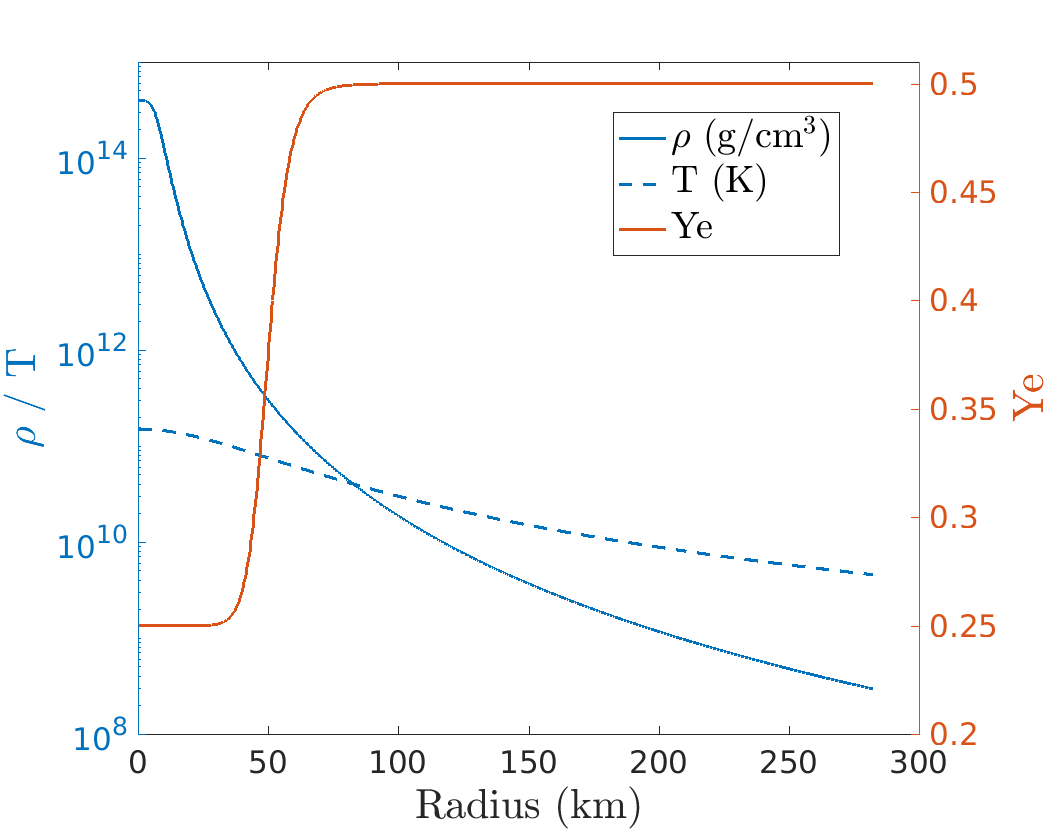
\includegraphics[width=0.45\textwidth]{figures/NStatinaryS_EOS}
    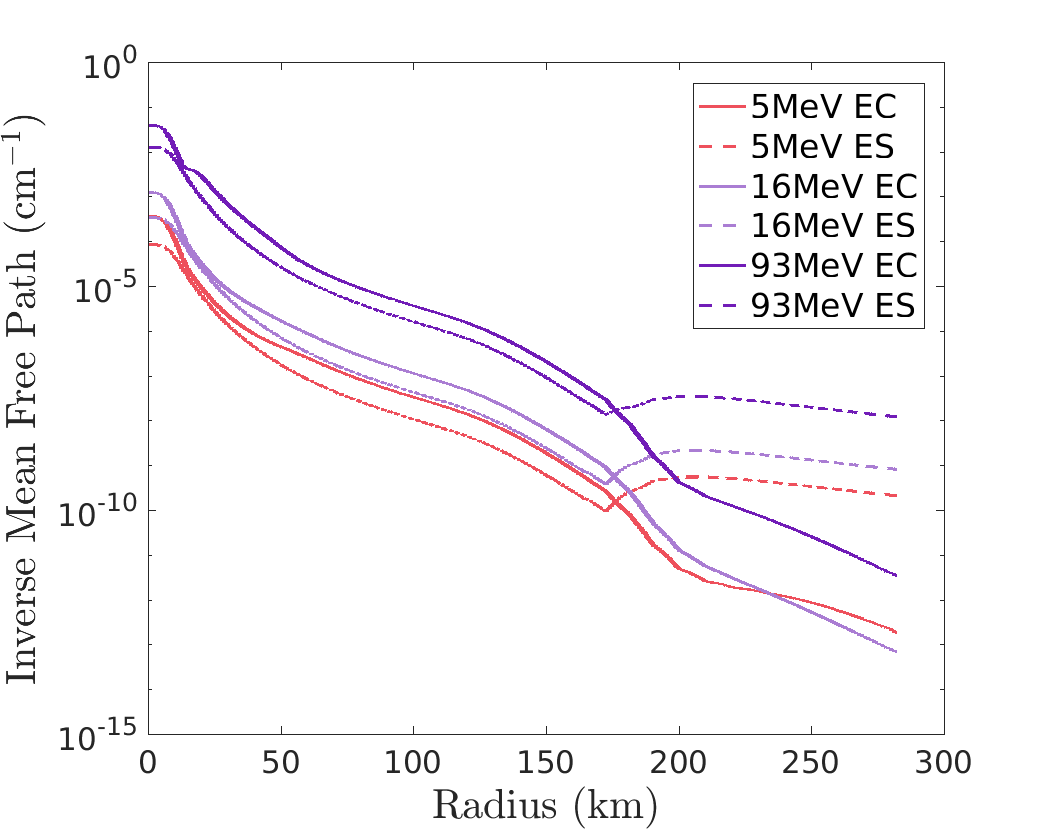
\includegraphics[width=0.45\textwidth]{figures/NSS_Opacities}
  \end{tabular}
   \caption{Thermal state (left) and neutrino absorptivity ($\sigma_{\Ab}$) and neutrino elastic scattering opacity ($ \sigma_{\Scatt}$) (right) for the neutrino stationary state test.}
   \label{fig:NeutrinoStationaryTestEOS}
\end{figure}

\begin{figure}[h]
  \centering
    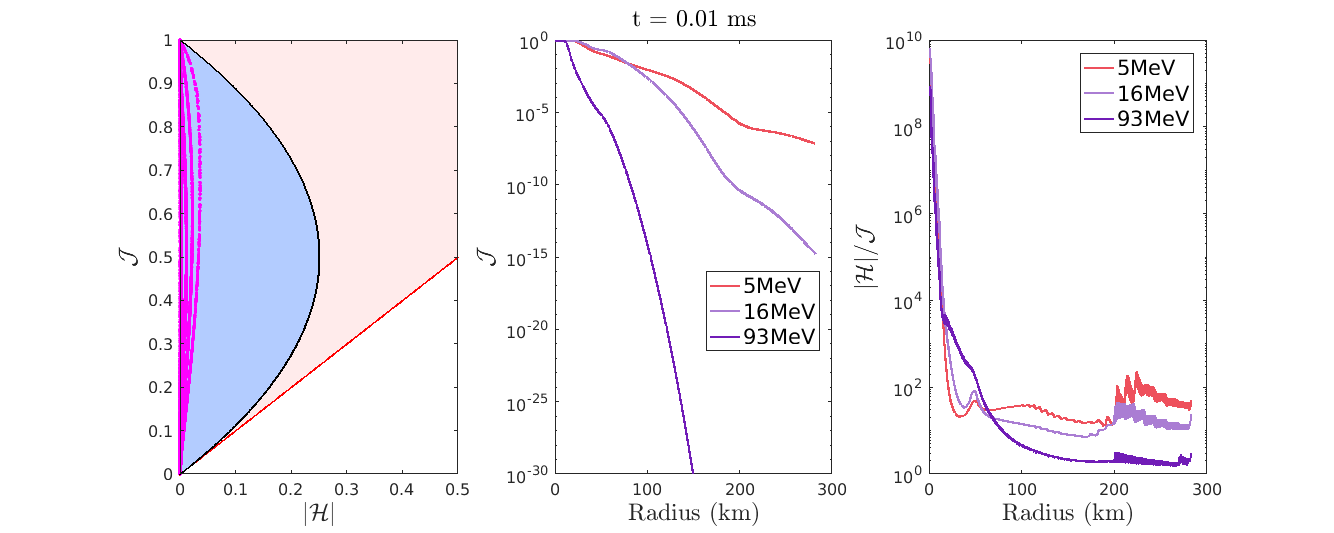
\includegraphics[width=\textwidth]{figures/NSS_1_1}\\
    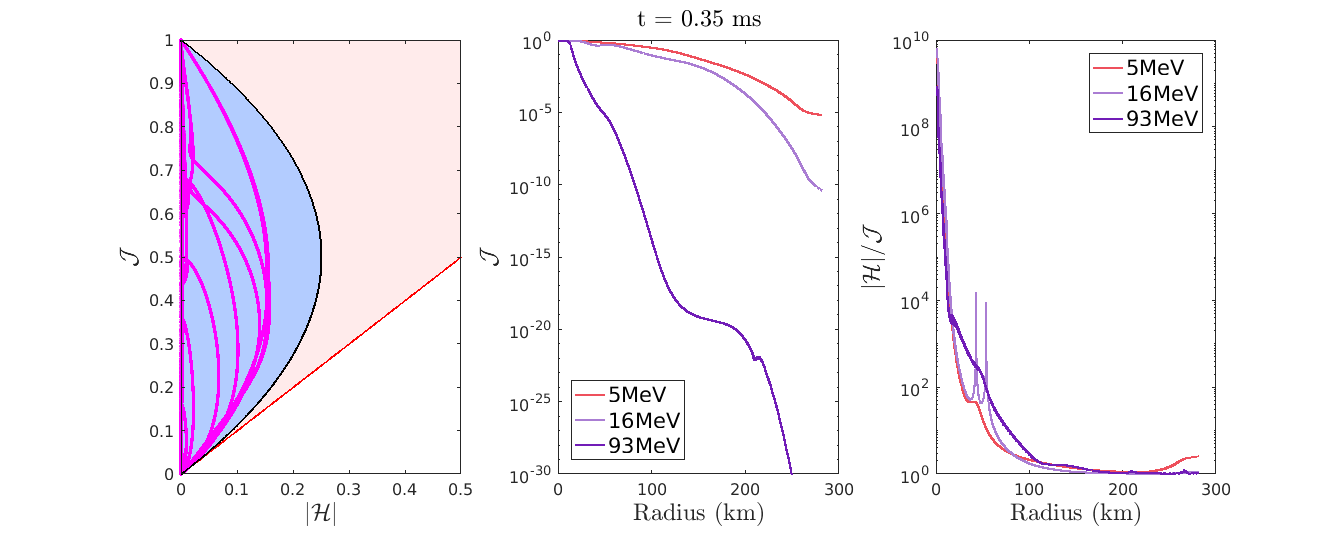
\includegraphics[width=\textwidth]{figures/NSS_3_1} \\
    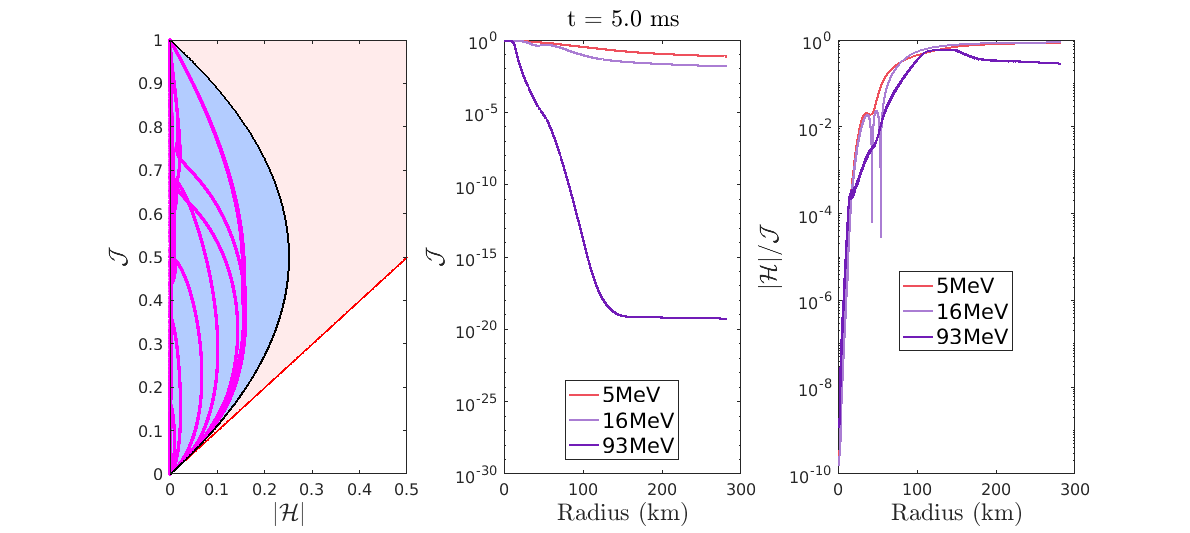
\includegraphics[width=\textwidth]{figures/NSS_5_1} \\
    \caption{Realizability (left column), the number density $\cJ$ versus radius (center column), and the flux factor $|\bcH|/\cJ$ versus radius (right column) at t = 0.01~ms ,0.35~ms and 5.0~ms for the neutrino stationary state test. For the realizability plots, the light blue area highlights the realizability domain, and the black lines define its boundary. Each $\bcM=(\cJ,\bcH)^{T}$ state is marked by a red dot. The results of PD-ARS with SSPRK2 and PD-ARS with SSPRK3 are indistinguishable in these plots.}
    \label{fig:NeutrinoStationaryTestEvolve}
\end{figure}

\clearpage